\chapter{Background} \label{chp:background}


\section{Compiler Infrastructure}

Compilers are programming tools responsible for translating programs in a given source language to a lower-level target language.
This compilation process must preserve the program semantics.
Moreover, compilers are also expected to produce a good quality representation of the program in the target language, optimising for a given objective function.
An important objective function is code size, i.e., the optimisation goal is to produce a representation of the program as small as possible.

%Compilers must preserve the program semantics.

In order to manage their complexity, compilers are usually designed in a highly modular manner, where they are organised as a series of phases that sequentially analyse and transform the program being compiled.
In their simplest form, compilers are usually organised in \textit{three-phases}, as shown in Figure~\ref{fig:3-phase-compiler}: frontend, optimiser, and backend.
The frontend is responsible for parsing, validating and diagnosing errors in the source code.
This parsed source code is then translated into an intermediate representation, which is the LLVM IR in this case.
The optimiser is responsible for doing a broad variety of transformations, that are usually independent of language and target machine, to improve the code's performance.
The backend, also known as the code generator, then translates the code from the intermediate representation onto the target instruction set.
It is common for the backend to also perform some low-level optimisations that take advantage of unusual features of the supported architecture.
%Common parts of a compiler backend include instruction selection, register allocation, and instruction scheduling.

\begin{figure}[h]
  \centering
  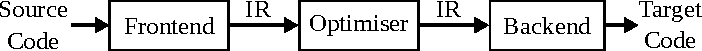
\includegraphics[scale=0.9]{src/background/figs/3-phase-compiler.pdf}
  \caption{Overview of the three-phase compiler infrastructure.}
  \label{fig:3-phase-compiler}
\end{figure}

%The front end parses source code, checking it for errors, and builds a language-specific Abstract Syntax Tree (AST) to represent the input code. The AST is optionally converted to a new representation for optimization, and the optimizer and back end are run on the code.
%The optimizer is responsible for doing a broad variety of transformations to try to improve the code's running time, such as eliminating redundant computations, and is usually more or less independent of language and target.


\begin{figure}[h]
  \centering
  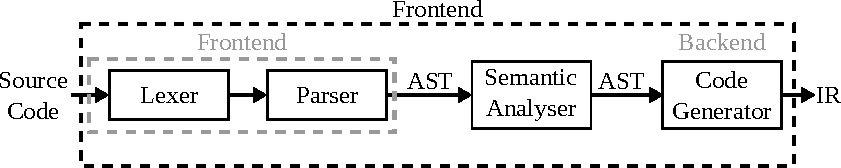
\includegraphics[scale=0.9]{src/background/figs/compiler-frontend.pdf}
  \caption{Overview of the three-phase compiler infrastructure.}
  \label{fig:compiler-frontend}
\end{figure}

\begin{figure}[h]
  \centering
  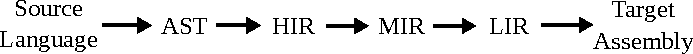
\includegraphics[scale=0.9]{src/background/figs/ir-lowering-sequence.pdf}
  \caption{Overview of the three-phase compiler infrastructure.}
  \label{fig:ir-lowering-sequence}
\end{figure}

\subsection{Link-Time Optimisations}
%% benefits of LTO
%% challenges with LTO
%% mention partial LTO, such as ThinLTO

\begin{figure}[h]
  \centering
  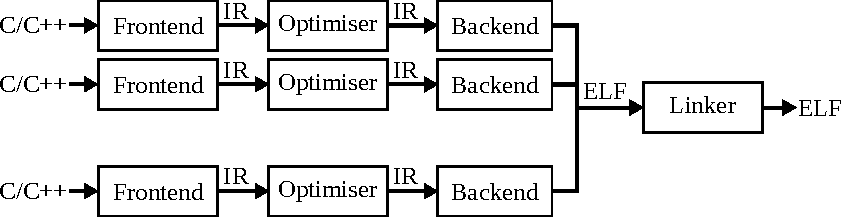
\includegraphics[scale=0.85]{src/background/figs/full-pipeline.pdf}
  \caption{Overview of the three-phase compiler infrastructure.}
  \label{fig:ir-lowering-sequence}
\end{figure}

\begin{figure}[h]
  \centering
  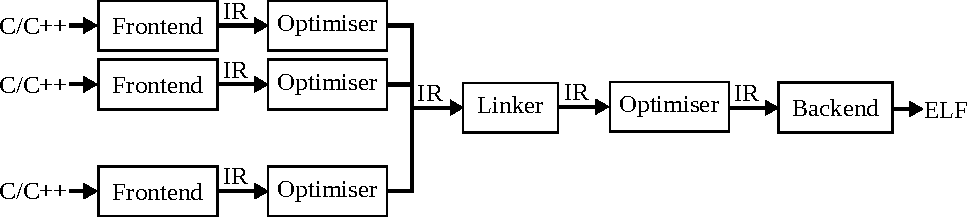
\includegraphics[scale=0.85]{src/background/figs/full-pipeline-LTO.pdf}
  \caption{Overview of the three-phase compiler infrastructure.}
  \label{fig:ir-lowering-sequence}
\end{figure}


%\section{Optimisation Scope}
%% describe local optimisations (block level), global (intra-procedural), and inter-procedural (across functions)

%\subsection{Interprocedural Optimisations}
%% benefits of IPO
%% challenges involved in IPO



\section{Sequence Alignment}

The comparison of two or more sequences, measuring the extent to which they differ, is important in many scientific areas, most notably in molecular biology~\cite{needleman70,smith81,carrillo88,wang94} where it has been critical
in the understanding of functional, structural, or evolutionary relationships between the sequences~\cite{kruskal83,mount05book}.

A particularly important comparison technique is sequence alignment, which identifies a series of patterns that appear in the same order in the sequences.
Essentially, sequence alignment algorithms insert blank characters in both input sequences so that the final sequences end up having the same size, where equivalent segments are aligned with their matching segments from the other sequence and non-equivalent segments are either paired with the blank or a mismatching character.

Figure~\ref{fig:seq-align-example} shows an example of a pair-wise sequence alignment.
This example, adapted from Lee~et~al.~\cite{lee02}, shows two protein sequences where amino acids are represented by their one-letter symbology~\cite{aasland68}.

\begin{figure}[h]
  \centering
  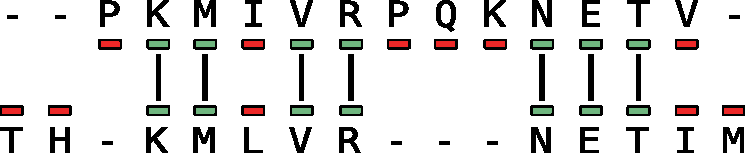
\includegraphics[scale=0.55]{src/background/figs/seq-align-example}
  \caption{Example of an optimum alignment between two sequences.
  Matching segments are shown in green, vertically centred, and the non-matching segments are shown in red at the sides.}
  \label{fig:seq-align-example}
\end{figure}

Formally, sequence alignment can be defined as follows:
For a given alphabet $\alpha$, a sequence $S$ of $k$ characters is an element of
$\alpha^k$, i.e., $S = (a_1, \ldots a_k)$.
Let $S_1, \ldots, S_m$ be a set of sequences, possibly of different lengths but
all derived from the same alphabet $\alpha$, where
$S_i = (a_1^{(i)}, \ldots, a_{k_i}^{(i)})$, for all $i\in\{1,\ldots,m\}$.
Consider an extended alphabet that includes the \textit{blank} character ``$-$'',
i.e., $\beta = \alpha \cup \{-\}$.
An alignment of the $m$ sequences, $S_1, \ldots, S_m$, is another set of sequences,
$\bar{S}_1, \ldots, \bar{S}_m$, such that each sequence $\bar{S}_i$ is obtained
from $S_i$ by inserting blanks in positions where some of the other sequences
have non-blank and possibly equivalent characters, for a given equivalence relation.
All sequences $\bar{S}_i$ in the alignment set have the same length $l$, where
$\max\{k_1,\ldots,k_m\} \leq l \leq k_1 + \cdots + k_m$.
Moreover, $\forall i\in\{1,\ldots, m\}$, $\bar{S}_i = (b_1^{(i)},\ldots,b_l^{(i)})$,
there are increasing functions $v_i: \{1,\ldots,k_i\} \to \{1,\ldots,l\}$, such that:
\begin{itemize}
\item $b_{v_i(j)}^{(i)} = a_j^{(i)}$, for every $j \in \{1,\ldots,k_i\}$;
\item any position not covered by the function $v_i$ contain a black character, i.e., for every $j \in \{1,\ldots,l\}\setminus \textrm{Im} \, v_i$, $b_j$ is the blank character ``$-$''.
\end{itemize}
Finally, for all $j\in\{1,\ldots,l\}$, there is at least one value of $i$ for which $b_j^{(i)}$ is not a blank character.
Note that two aligned sequences may contain both non-blank and non-equivalent characters at any given position, in which case there is a mismatch.

The sequence alignment problem is concerned with identifying an alignment that maximises the score for a given scoring scheme.
The scoring scheme first defines a weight for the alignment of pairs of characters which will then be used to compose a score for the whole sequence alignment.
These weights are used to penalise mismatches and gaps while favouring matching pairs.

The alignment score between two characters is defined by a function on pairs of characters, $\delta \in \beta\times\beta \to \mathbb{R}$, for a given extended alphabet $\beta$.
The simplest function that is commonly used is the constant function~\cite{haque09}.
Let $a,b\in\beta$ and $a \neq b$.
This constant function is defined by a triple $(w_1,w_2,w_3)\in\mathbb{R}^+\times\mathbb{R}^-\times\mathbb{R}^-$, such that:
\begin{itemize}
\item For two matching caracters, $\delta(a,a) = w_1, w_1\in\mathbb{R}^+$.
\item For a mismatch betweem non-blank characters, $\delta(a,b) = w_2, w_2\in\mathbb{R}^-$.
\item The gap penalty, for when we have a blank character, $\delta(a,-) = \delta(-,a) = w_3, w_3\in\mathbb{R}^-$.
\end{itemize}
This is a simple scoring scheme that rewards matches and penalises mismatches and gaps.

There is a vast literature on algorithms for performing sequence alignment, especially in the context of molecular biology.
These algorithms are classified as either global or local.
A global sequence alignment algorithm attempts to align the entire sequence, using as many characters as possible, up to both ends of each sequence.
Global alignment algorithms are useful for sequences that are highly similar and have approximately the same length~\cite{mount05book}.
Alternatively, a local sequence alignment algorithm generates subalignments in stretches of sequence with the highest density of matches.
Local alignments are more suitable for aligning sequences with very few similarities or vastly different lengths~\cite{mount05book}.

In this work, we will focus on pair-wise global alignment algorithms.
The following sections describe the main optimal algorithms based on dynamic programming.
These algorithms will offer different optimality, performance, and memory usage trade-offs~\cite{needleman70,smith81,carrillo88,hickey11}.
%Different alignments would produce different but valid merged functions.

\subsection{Needleman-Wunsch Algorithm}

The Needleman-Wunsch algorithm~\cite{needleman70} is one of the most well known algorithm for pair-wise global alignment.
This algorithm gives an alignment that is guaranteed to be optimal for a given scoring scheme~\cite{higgins89}.

The Needleman-Wunsch algorithm is based on dynamic programming and consists of two main steps.
First, it builds a \textit{similarity matrix}, based on a scoring scheme, which assigns weights for matches, mismatches, and \textit{gaps} (blank characters).
Afterwards, a backward traversal is performed on the similarity matrix, in order to reconstruct the final alignment by maximizing the total score.

\begin{figure}[h]
  \centering
  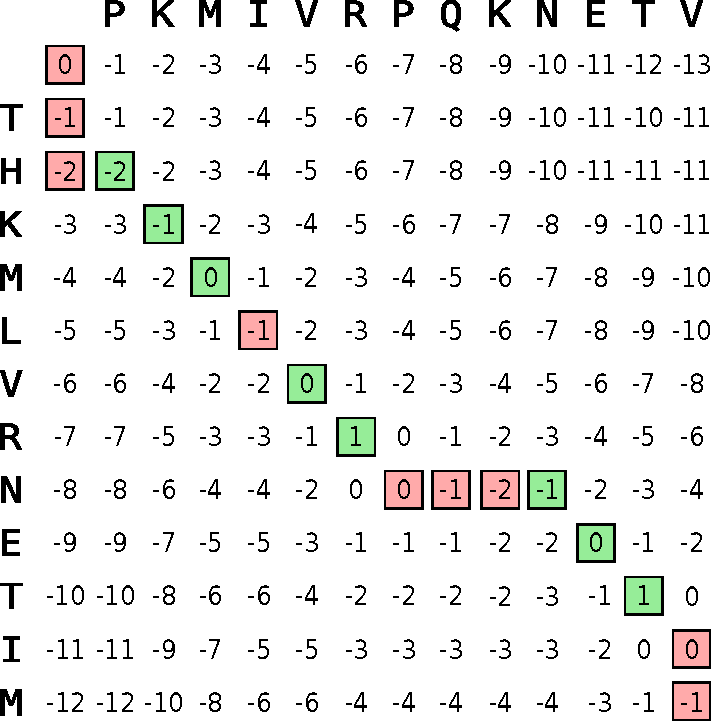
\includegraphics[scale=0.6]{src/background/figs/seq-align-example-nw}
  \caption{Example of the \textit{similarity matrix} computed for two input sequences.
           The highlighted cells represent the resulting alignment computed by the Needleman-Wunsch algorithm.}
  \label{fig:seq-align-example-nw}
\end{figure}

Figure~\ref{fig:seq-align-example-nw} shows the similarity matrix corresponding to the example from Figure~\ref{fig:seq-align-example}.
The similarity matrix is constructed by comparing all possible pairs of characters from the input sequences.
Let $S_1$ and $S_2$ be our input sequences of sizes $k_1$ and $k_2$, respectively, where $S_1 = (a_1,\ldots,a_{k_1})$ and $S_2 = (b_1,\ldots,b_{k_2})$.
The similarity matrix $M$ computed for these two input sequences will have size $(k_1 + 1) \times (k_2+1)$.
Let $M_{i,j}$ denote all entries in the similarity matrix, with $1 \leq i \leq (k_1 + 1)$ and $1 \leq j \leq (k_2 + 1)$.
The first entry in the matrix is $M_{1,1} = 0$, and
\begin{equation*}
%\begin{align*}
M_{i,j} = \max \begin{cases}
  M_{i-1,j} + \delta(a_{i-1},-)         &  \quad  \text{if } i>1 \text{ and } j\geq1 \\
  M_{i,j-1} + \delta(-,b_{j-1})         &  \quad  \text{if } i\geq1 \text{ and } j>1 \\
  M_{i-1,j-1} + \delta(a_{i-1},b_{j-1}) &  \quad  \text{if } i>1 \text{ and } j>1
\end{cases}
%\end{align*}
\end{equation*}
In other words, the score for each cell in the similarity matrix is the maximum among the rules shown in Figure~\ref{fig:seq-align-rules}.

\begin{figure}[h]
  \centering
  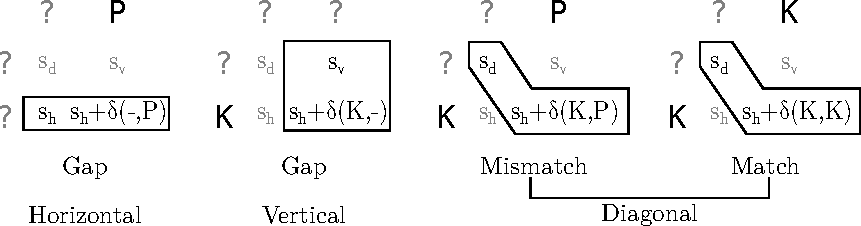
\includegraphics[scale=0.8]{src/background/figs/seq-align-rules}
  \caption{Set of rules used to compute the scores of the similarity matrix.
           The two first rules represent the penalty of inserting a horizontal or vertical gap.
           The diagonal rule depends whether we have a matching or mismatching pair of input characters.}
  \label{fig:seq-align-rules}
\end{figure}


Figure~\ref{fig:seq-align-example-nw} also highlights the traversal. 
Note that sometimes, while traversing the score matrix, there are multiple adjacent neighbours with the same score.
Since there may exist multiple traversals with the same score, two sequences can have multiple optimum alignments.

Needleman-Wunsh algorithm is quadratic in the size of the sequences being aligned, both in time and space.

%\subsection{Hirschberg Algorithm}


\section{Machine Learning}

Machine learning (ML) is the field of study of mathematical models that can automatically learn patterns from sample data, known as \textit{training} data, in order to make predictions for unseen data.
Regression and classification are two common types of machine learning application~\cite{goodfellow16}.

Regression concerns the prediction of a numerical value given some inputs, where an ML model learns the relationship between the outcome variable and one or more input features.
Figure~\ref{fig:ml-regression} illustrates an example of a regression model.
Based on the sample data, a curve is fitted, minimising the overall error between the sample data and the curve.
This curve represents the model that can be used to estimate the outcome variable for an unseen feature data.

\begin{figure}[h]
  \centering
  \begin{subfigure}{.32\textwidth}
    \center
    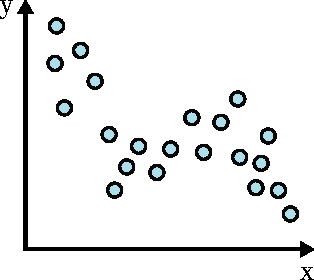
\includegraphics[scale=0.8]{src/background/figs/ml-regression-sample}
    \caption{Sample data.}
    \label{fig:ml-regression-sample}
  \end{subfigure}
  \begin{subfigure}{.32\textwidth}
    \center
    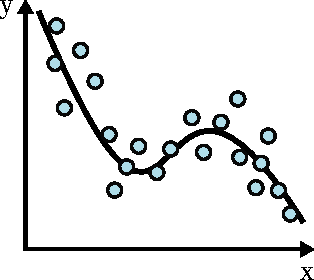
\includegraphics[scale=0.8]{src/background/figs/ml-regression-fitted}
    \caption{Fitted curve.}
    \label{fig:ml-regression-fitted}
  \end{subfigure}
  \begin{subfigure}{.32\textwidth}
    \center
    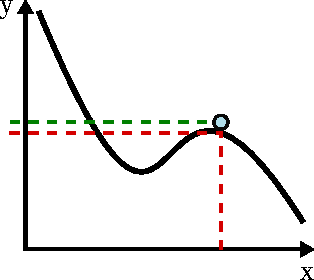
\includegraphics[scale=0.8]{src/background/figs/ml-regression-model}
    \caption{Model.}
    \label{fig:ml-regression-model}
  \end{subfigure}
  \caption{
    An illustration of a regression model using machine learning.
    A regression model use the sample data to learn a function that maps the input features to an outcome numerical variable.
  }
  \label{fig:ml-regression}
\end{figure}

Classification concerns the prediction of a categorical label given some inputs, where an ML model learns the relationship between a finite set of labels and one or more input features.
The training of a classifier requires inputs for which the category is known, called labelled training data.
Figure~\ref{fig:ml-classifier} illustrates an example of a binary classification model.
Based on the sample data, a curve is fitted, minimising the number of misclassification.
This curve represents the model that can be used to predict the category of unseen feature data.

% In this type of task, the computer program is asked to specify which of k categories some input belongs to. To solve this task, the learning algorithm is usually asked to produce a function f:Rn→ {1, . . . , k}. When y=f(x), the model assigns an input described by vector x to a category identified by numeric code y. There are other variants of the classification task, for example, where f outputs a probability distribution over classes. An example of a classification task is object recognition, where the input is an image (usually described as a set of pixel brightness values), and the output is a numeric code identifying the object in the image.

\begin{figure}[h]
  \centering
  \begin{subfigure}{.32\textwidth}
    \center
    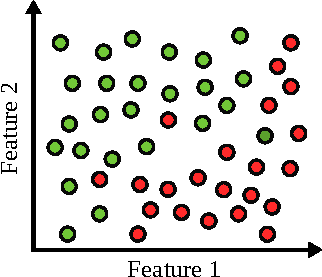
\includegraphics[scale=0.8]{src/background/figs/ml-classifier-sample}
    \caption{Sample data.}
    \label{fig:ml-classifier-sample}
  \end{subfigure}
  \begin{subfigure}{.32\textwidth}
    \center
    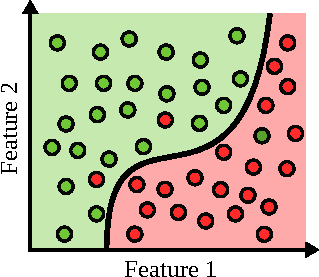
\includegraphics[scale=0.8]{src/background/figs/ml-classifier-fitted}
    \caption{Fitted curve.}
    \label{fig:ml-classifier-fitted}
  \end{subfigure}
  \begin{subfigure}{.32\textwidth}
    \center
    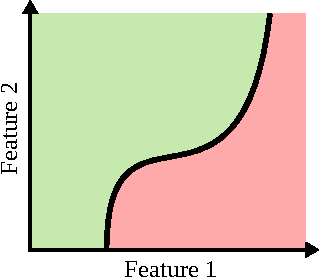
\includegraphics[scale=0.8]{src/background/figs/ml-classifier-model}
    \caption{Model.}
    \label{fig:ml-classifier-model}
  \end{subfigure}
  \caption{
    An illustration of a classification model using machine learning.
    A regression model use the sample data to learn a function that maps the input features to an outcome numerical variable.
  }
  \label{fig:ml-classifier}
\end{figure}

\subsection{Neural Networks}

Machine is commonly seen as a subset of artificial intelligence and a superset of deep-learning (DL), which is a family of machine learning methods based on artificial neural networks.
Artificial neural networks (ANNs) are machine learning models that were vaguely inspired by the biological neural networks.
These models are composed of artificial neurons, which are essentially mathematical functions known as \textit{activation functions}, mapping inputs to a single output that can be fed to multiple other neurons.
These neurons are connected by weighted edges, forming a graph, i.e., the artificial neural network.

\subsubsection{Feed-Forward Neural Networks}

A feed-forward neural networks is a simple but powerful neural network architecture where information flows through the layers in only one direction, namely, forward, as illustrated in Figure~\ref{fig:ML-feed-forward-network}.
Feed-forward neural networks with multiple layers work as universal function approximators of any bounded continuous function to arbitrary precision~\cite{hornik91,lu17}.
Essentially, this model defines a mapping $\mathbf{y} = f(\mathbf{x};\mathbf{\theta})$, were $\mathbf{\theta}$ represents the parameters that are learnt, optimising the function approximation.

The architecture of the feed-forward network is a direct acyclic graph, where the neurons are grouped in layers, forming what is also known as a multi-layer perceptrons.
The neurons are connected only across layers, i.e., the neurons in one layer are connect to the neurons following layer.
The first layer is the input layer, with $x_i$ being the input variables, and the last layer is the output layer, with $y_i$ being the output variables.
All other layers in between are the hidden layers, for which there are no known ground truth values.
The value for these hidden layers are computed using a specific activation function that is chosen per layer.
The number of layers of the architecture is known as the depth of the model, with the final layer being the output layer.
When designing the architecture of a feed-forward neural network, in addition to the activation functions in each layer, we must also decide on how many layers the network should contain, how these layers should be connected to each other, and how many units should be in each layer~\cite{goodfellow16}.

\begin{figure}[h]
  \centering
  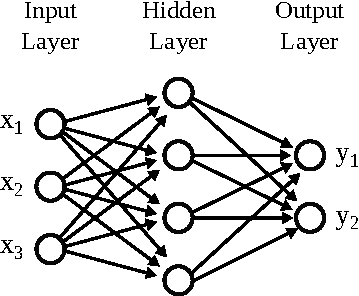
\includegraphics[scale=0.85]{src/background/figs/ML-feed-forward-network.pdf}
  \caption{Example of an artificial neural network with multiple layers of neurons. Each circle represents an artificial neuron. Adjacent layers of neurons are fully connected.}
  \label{fig:ML-feed-forward-network}
\end{figure}

%\paragraph{Activation Function}

%A common activation function in feed forward networks are sigmoids.
%Two of the sigmoid functions commonly used are the logistic and the hyperbolic tangent function.
%The logistic function is defined as $\phi(x) = \frac{1}{1+e^{-x}}$ and the hyperbolic tangent function is defined as 

\paragraph{Back-propagation}

Neural networks can use a large variety of learning algorithms.
Learning consists of finding weights for the parameters in order to minimise the prediction error.
The most widely used learning technique is known as back-propagation~\cite{rumelhart88,goodfellow16}.

Learning in deep neural networks requires computing the gradients of complicated functions.
We present the back-propagation algorithm and its modern generalizations, which can be used to efficiently compute these gradients.

Typically, this algorithm initialises the weights with random values.
During the training process, a batch of samples is propagated through the network in a feed-forward way.
The outputs of the network is then compared against the true values, computing a prediction error.
The error function is chosen as part of the design of the network, as the appropriate function depends on the task.
This prediction error is propagated back to each individual neuron. %, using the learning rule below:

For each neuron, it computes what the output should have been and updates the weights of the neuron accordingly.
Finally, this process is repeated for different batches until it converges, producing a prediction error below a certain threshold.

\subsubsection{Recurrent Neural Networks}

Recurrent neural networks (RNNs) are a family of neural networks for processing sequential.
Most recurrent networks can process sequences of variable length, which is impractical for networks without sequence-based specialisation.
In order to process input sequences of variable length, RNNs have feed-back connections in which outputs of the model are fed back into itself, forming a cycle (or recursion) in the network~\cite{goodfellow16}.

Two important RNNs are long short-term memory and networks based on the gated recurrent unit.

\paragraph{Long Short-Term Memory}

Long short-term memory~\cite{Graves12} (LSTM) is an RNN architecture designed to overcome the vanishing gradients problem.
The LSTM augments RNN design with the addition of a cell for storing information, and three gates which control the flow of information into and out of the cell.

Long short-term memory (LSTM) is an RNN architecture designed to overcome the vanishing gradients problem.
The LSTM augments RNN design with the addition of a cell for storing information, and three gates which control the flow of information into and out of the cell.

\paragraph{Gated Recurrent Units}

Gated recurrent units (GRUs) are a gating mechanism in recurrent neural networks, introduced in 2014 by Kyunghyun Cho et al. The GRU is like a long short-term memory (LSTM) with a forget gate but has fewer parameters than LSTM, as it lacks an output gate. GRU's performance on certain tasks of polyphonic music modeling, speech signal modeling and natural language processing was found to be similar to that of LSTM. GRUs have been shown to exhibit even better performance on certain smaller and less frequent datasets.

